\chapter{Theoretische Grundlagen}
Dieses Kapitel erläutert die Grundlagen die zum 
Verständnis dieser Arbeit notwendig sind. Zuerst werden bereits bestehende Technologien wie 
Docker und Kubernetes erklärt, dabei wird bausteinartig auf das Thema Microservices hingeführt.

%TEXT!!!!

\section{Docker}

In diesem Abschnitt wird die Technologie \glqq Docker\grqq{} näher erläutert und
nicht das Unternehmen \glqq Docker, Inc.\grqq{}, dass für die maßgebliche Entwicklung dessen verantwortlich ist.
Angefangen mit der Terminologie, zum deutlicheren Verständnis der nächsten Abschnitte.
Forgesetzt mit der aufsteigenden Erklärung der Architektur bis zum Aufbau eines Containers.

%\subsection{Terminologie}
%\begin{itemize}
%    \item \textbf{Container}: Isolierter Prozess mit einer laufenden Anwendung.
%    \item \textbf{Volumes}: Persistente Daten eines Containers.
%    \item \textbf{Image}: Einheit mit ausführbaren Code, Abhängigkeiten und Betriebssystem. Aufgeteilt in mehreren Schichten.
%    \item \textbf{Dockerfile}: Textdatei zum erstellen eines Docker-Images.    
%\end{itemize}

\subsection{Architektur}
Die Docker Technologie ist in der Programmiersprache \glqq GO\grqq{} geschrieben und nutzt Funktionalitäten des
Linux Kernels, wie cgroups und namespaces.
Namespaces ermöglichen die Isolation von Prozessen in sogenannte Container, welche unabhängig voneinander arbeiten \cite{dockergetstarted}.
Diese beeinhalten alle nötigen Abhängigkeiten zur Ausführung der vordefinierten Anwendung.
Container gewinnen dadurch an Portabilität, die ein bereitstellen auf Infrastrukturen mit der Docker
Laufzeit ermöglichen.
Die Laufzeit setzt sich aus \glqq runc\grqq{} einer low-Level Laufzeit und \glqq containerd\grqq{} einer higher-Level
Laufzeit zusammen (vgl. Abbildung~\ref{fig:dockerarch}).
Runc dient als Schnittstelle zum Betriebssystem und startet und stoppt Container.
Containerd verwaltet die Lebenszyklen eines Container, ziehen von Images, erstellen von Netzwerken und
Verwaltung von runc.
Die Allgemeine Aufgabe des Docker Daemons ist es eine vereinfachte Schnittstelle für die Abstraktion
der unterliegenden Schicht zu gewährleisten, wie zum Beispiel dem verwalten von Images, Volumes und Netzwerken \cite{dockerdeep}.
Auf die Orchestrierung mit Swarm wird nicht weiter eingeganen, da sie zum Verständnis nicht nötig ist.

\begin{figure}
    \centering
    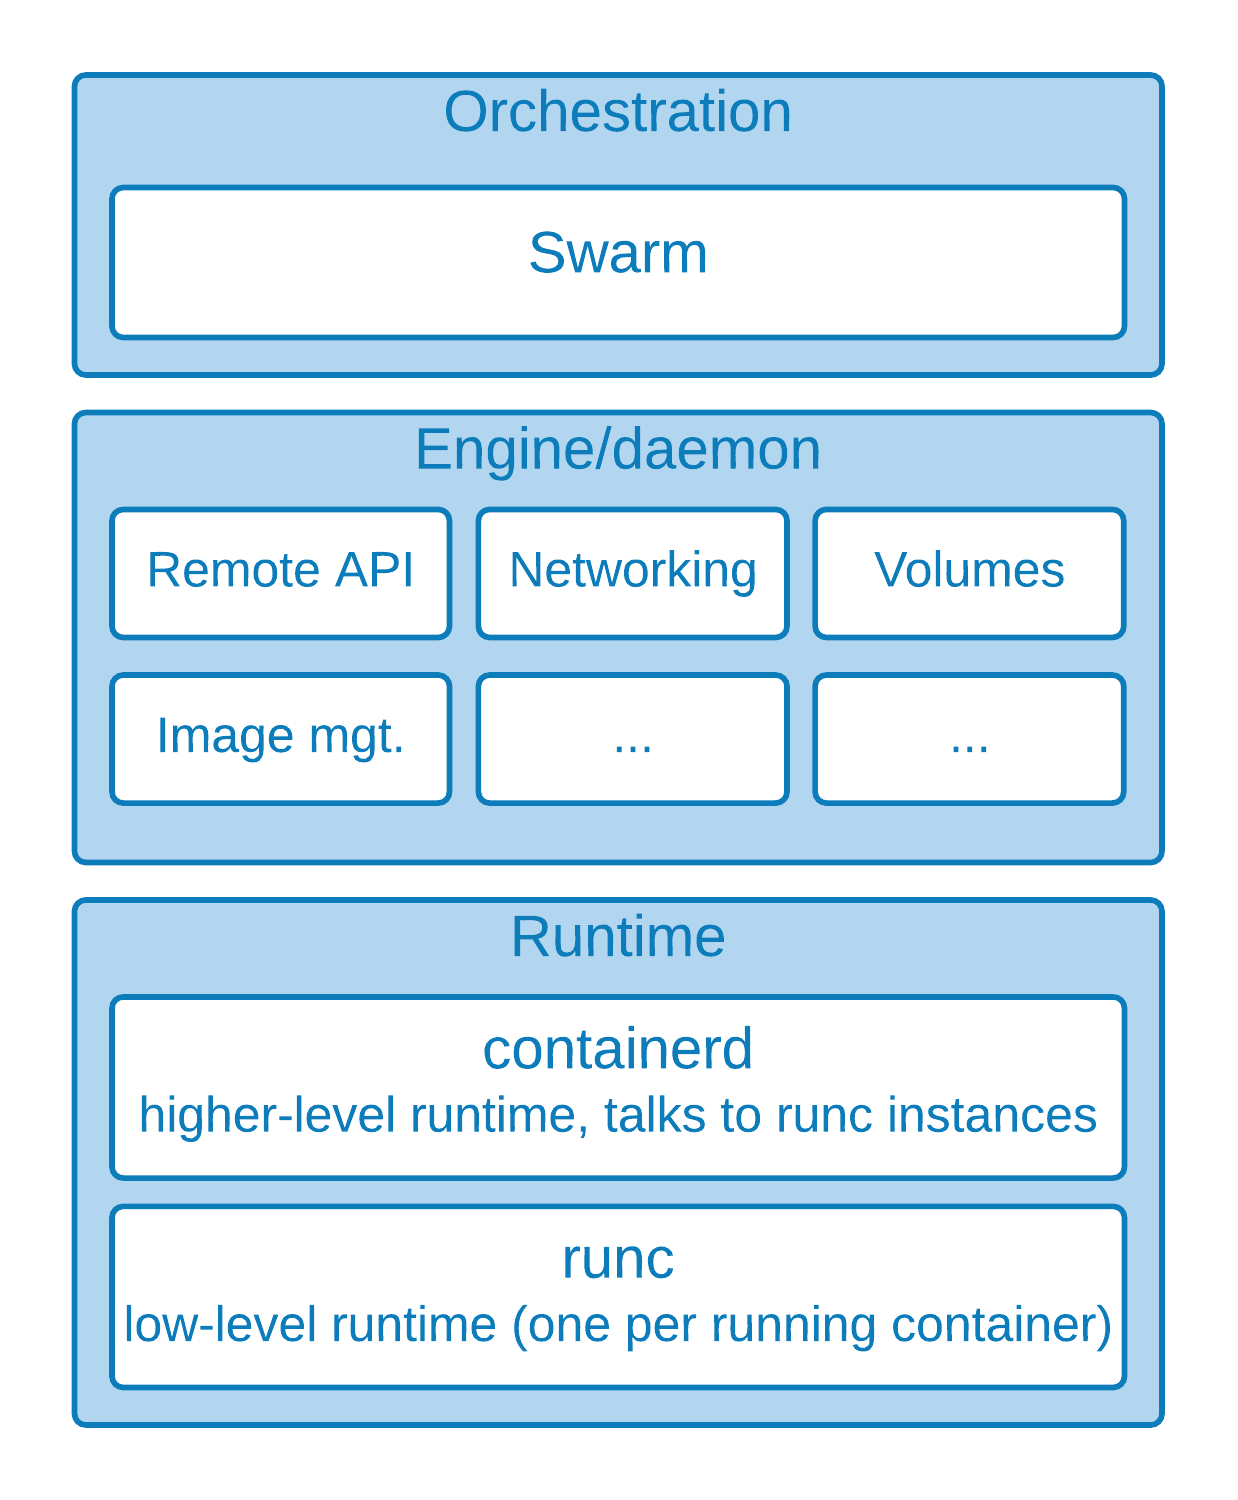
\includegraphics[width=0.5\columnwidth]{images/DockerArch.png}
    \caption{Docker Architektur \protect\cite{dockerdeep}}
    \label{fig:dockerarch}
\end{figure}

\subsection{Images und Container}
Ein Docker Image ist ein Objekt das alle Abhängigkeiten wie Quellcode, Bibliotheken und Betriebssystem
Funktionen für eine Anwendung beeinhaltet. 

\subsubsection{Registries}
Das beziehen von Images erfolgt über sogenannte \glqq Image Registries\grqq{}.
Bei Docker ist dies standardmäßig \url{https://hub.docker.com} und das eigene Lokale Registry. 
Es ist auch möglich eigene zu hosten oder die von Drittanbieter zu nutzen.

\subsubsection{Schichten}
Docker Images bestehen aus mehreren Schichten, jede davon abhängig von der Schicht unter ihr und
erkennbar durch IDs in Form von SHA256 Hashes (vgl. Abbildung~\ref{fig:dockerlayer}).
Docker kann dadurch beim bauen oder updaten von neuen Images vorhandene Schichten erneut verwenden. 
Die feste Reihenfolge ermöglicht eine ressourceneffiziente Verwaltung von Builds,
indem man oft wechselnde Schichten oben platziert. 
Die Leistung beim erstellen und zusammenführen von Schichtem hängt vom Dateisystem des Hostsystems ab.
Eine Schicht kann aus mehreren Dateien bestehen
und einzelne Dateien aus der Unterliegenden Schicht mit einer neuen ersetzen.

\begin{figure}
    \centering
    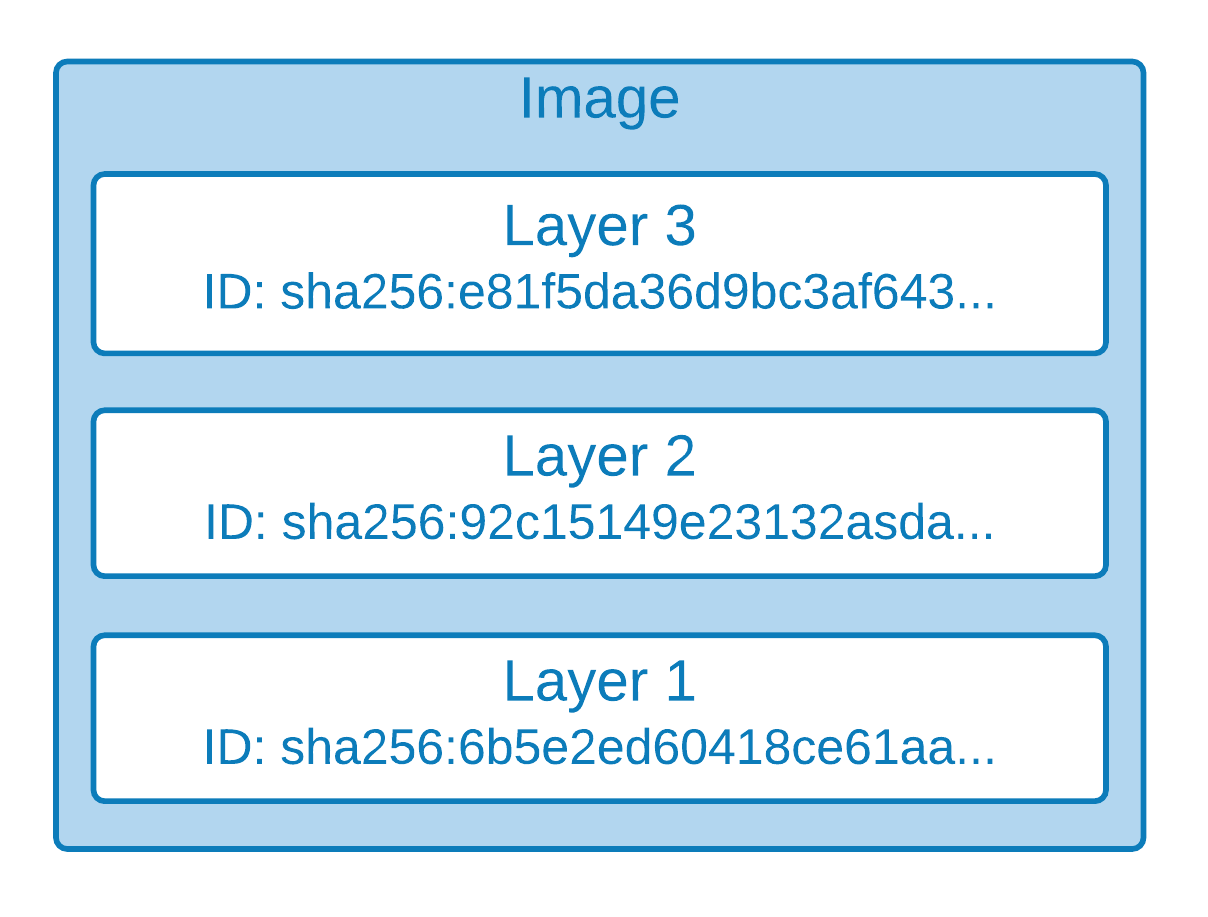
\includegraphics[width=0.5\columnwidth]{images/Image-Layer.png}
    \caption{Image Layers \protect}
    \label{fig:dockerlayer}
\end{figure}

%copy-on-write (CoW) strategy???

%nicht alle dockerfile anweisungen erstellen layer ENV expose usw.
Das starten eines Containers fügt auf die bereits bestehenden Schichten einen \glqq Thin R/W layer\grqq{} 
oder auch \glqq Container layer\grqq{} genannt hinzu, dieser gewährt Schreib- und Leserechte bei Laufzeit des Prozesses. 
Jeder dieser Container hat somit einen individuellen Zustand, der unähnlich vom abstammendem Image ist.
Bei Löschung des Containers verschwindet auch die dazu gewonne Schicht.
Das entfernen eines Images ist durch die Konzeption des Schichtensystem erst möglich, wenn alle darauf
basierenden Container gelöscht sind \cite{dockerstoragedriver}.

\subsubsection{Dockerfile}
Zur Erstellung eines Docker Images wird ein Dockerfile benötigt, dies beeinhaltet alle Anweisungen
zum Aufbau der einzelnen Schichten.

\subsection{Containervirtualisierung}
Ein Container ist eine laufende Instanz eines Images.



Dieses Konzept kommt dem einen oder anderen Leser vielleicht schon bekannt vor,
vergleichbar ist dieses Konzept mit dem einer VM.
Images ermöglichen ähnlich wie VM templates,das erstellen von mehreren Instanzen durch eine Vorkonfiguration.
Mit dem großen Unterschied, dass die Einrichtung von VMs müheseliger ist und weitaus mehr Ressourcen
beansprucht, da sie ein ganzes Betriebssystem ausführt. Containertechnologien bauen hingegen nur auf 
bestimmte Funktionalitäten des Kernels auf und sparen damit an Rechenleistung (vgl. Abbildung~\ref{fig:containervm}).

\begin{figure}
    \centering
    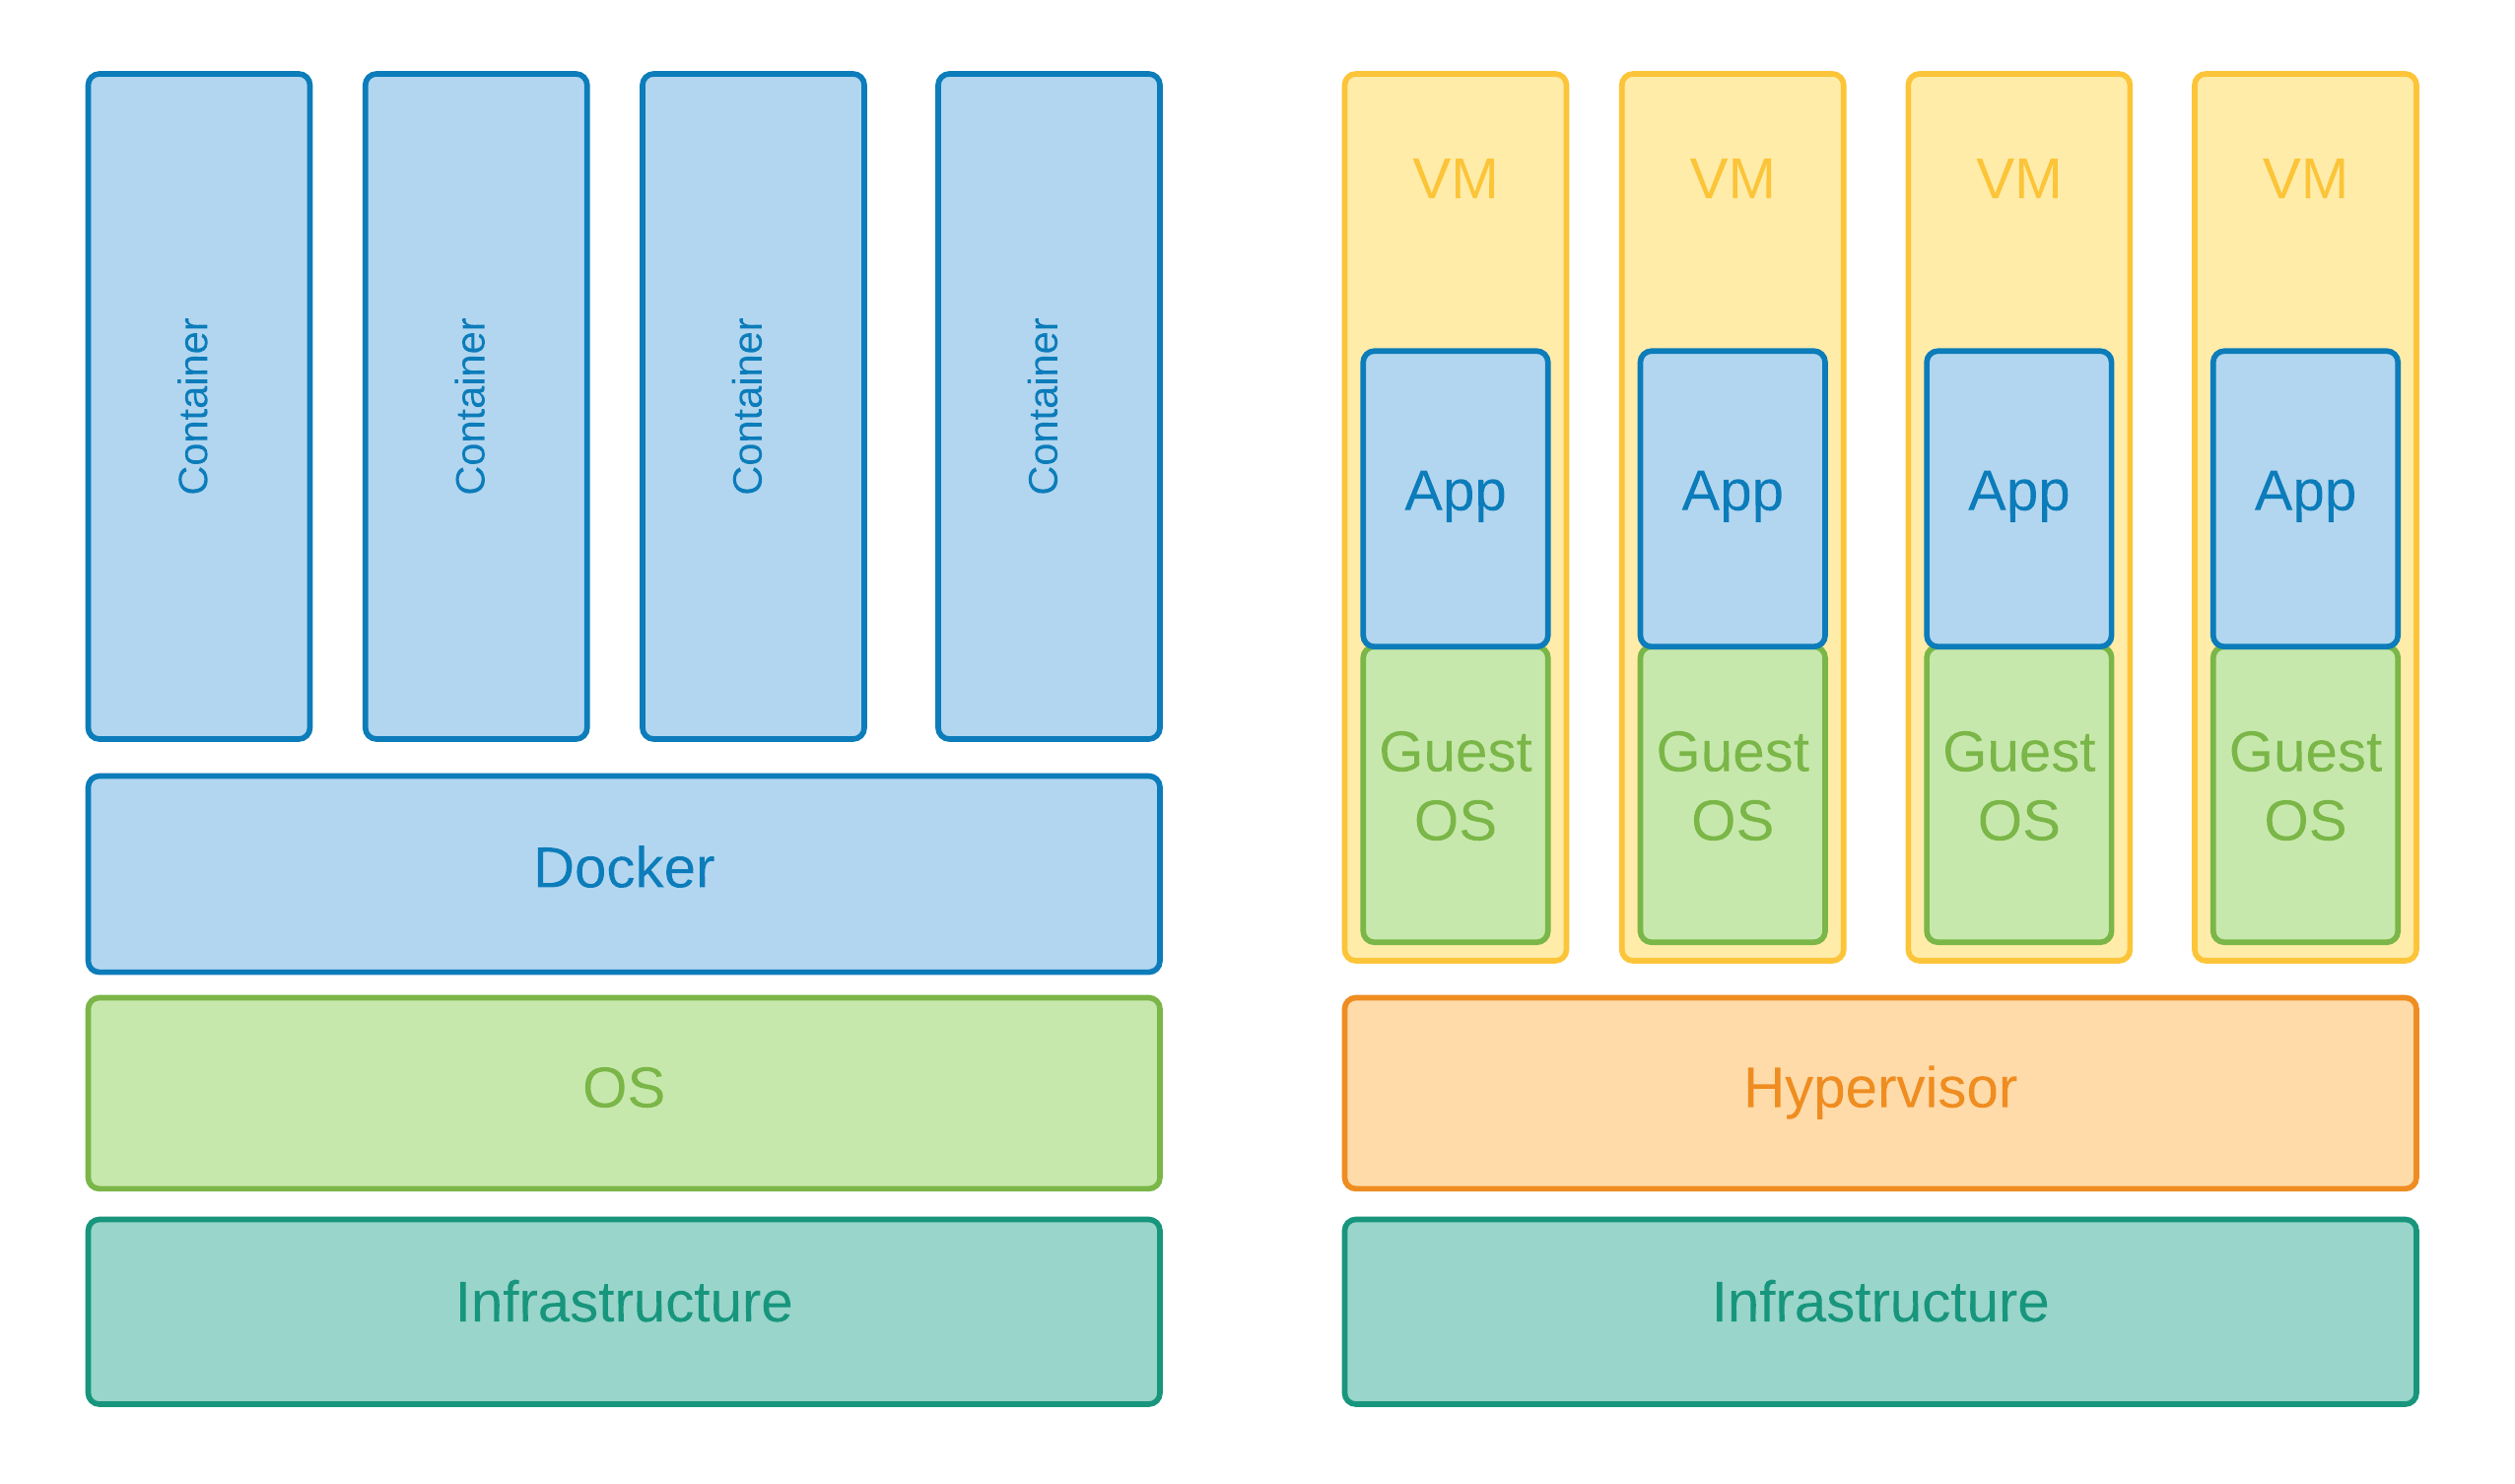
\includegraphics[width=1.0\columnwidth]{images/Container-VM.png}
    \caption{Container gegen virtuelle Maschinen \protect}
    \label{fig:containervm}
\end{figure}

\section{Kubernetes}
\subsection{Architektur}
\subsection{Lightweight Kubernetes}
\subsection{Hybrid Cloud}
\subsection{Rancher}

\section{Microservice}
\subsection{Aufbau}
\subsection{Entwicklung}
\subsection{Dezentrale Datenmanagement}





%\subsubsection{Ein Unterabschnitt}
